\chapter{Analytic model of nondegenerate internal squeezing} %Research chapter: ...
\label{chp:nIS_analytics}

% results: interpret deep and far, and be very critical of assessing your approach
% present analysis of model and decisions/approximations made
% think about the story!
% systematic and diligent
% wring all of the information out of the results/figures, find the importance and the physics

% separate this into multiple .tex files once structure finalised

%%%%%%%%%%%%%%%%%%%%%%%%%%%%%%%%%%%%%%%%%%
% chapter introduction

\jam{(Fix up mentions of nondegenerate internal squeezing in background chapters, either explain it earlier or do not confuse the reader)}

% combine the all-optical approach of dIS with the mode structure of sWLC
In this chapter, I present my analytic, Hamiltonian model of nondegenerate internal squeezing and the immediate results from it. Nondegenerate internal squeezing is the same configuration as degenerate internal squeezing except that the squeezer is operated nondegenerately, but it is better thought of as an all-optical alternative to stable optomechanical filtering. Firstly, I will review the limited literature available about nondegenerate internal squeezing, and conclude that the system with optical loss has never been fully characterised. Secondly, I will present my model and derive the sensitivity of the configuration. Thirdly, I will partially verify the model by demonstrating that it obeys the expected low and high loss limits. Fourthly, I will show that the system is stable by examining the zeros of the transfer functions' denominator. And finally, motivated by the sensitivity analysis, I will derive the threshold of the lossy configuration using an observation that unites the different squeezing configurations in this thesis. 
% from the view of quantum optics, gravitational waves in the next chapter
This chapter is written from the perspective of understanding nondegenerate internal squeezing for general quantum metrology. In the following chapters, I will return to the problem of kilohertz gravitational-wave detection and whether nondegenerate internal squeezing can improve sensitivity. 


\section{Literature review}
% a gap in the literature, should be much shorter than the review in Section~\ref{sec:literature_review} -- maybe combine it with that one?
% cannot cite personal communication?
% claim: the modelling of this configuration has never been done as thoroughly as my work, explain why (recency of interest)

\jam{(How to be thorough with this section?)}

The available literature about nondegenerate internal squeezing is limited. Although nondegenerate OPOs have long been studied for tests of the EPR-paradox~\cite{Reid1989,Schori2001} and other applications~\cite{,,}, placing a nondegenerate squeezer in a coupled cavity system \jam{has only been studied in ... (I am not aware of any other mentions than Li 2020, need to read up and ask the supervisors.)}. 
The two configurations in the previous chapter which motivate nondegenerate internal squeezing have only recently \jam{(quantify this?)} been studied, see Section~\ref{sec:literature_review}, and a study of nondegenerate internal squeezing seems inevitable to follow from combining those configurations. \jam{(Is there direct mention of nIS in the dIS literature?)}
The only direct mention of nondegenerate internal squeezing \jam{(that I could find, check this!)} in the literature is the brief suggestion in Ref.~\cite{Li2020} that it is equivalent to stable optomechanical filtering in the lossless case. In that paper, and subsequent work by the same authors~\cite{Li2021}, only mechanical loss is included in the model since it is the dominant source of loss. By the modal equivalence, I predict that optical loss in the idler mode should be the dominant source of loss for nondegenerate internal squeezing, but this is not guaranteed because the behaviour of mechanical and optical loss is different~\cite{} \jam{(is it? but same Langevin terms?)}. I identify this as a gap in the literature, no work has fully characterised the behaviour of the three mode system in the presence of optical loss in every mode, which matters because the distribution of loss in applications might be far from uniform, e.g.\ how the detection loss is predicted to be higher than any of the intra-cavity losses for future gravitational-wave detectors~\cite{}. By a full characterisation, I mean that not only is the quantum noise and signal response of the lossy system not available, but aspects important to understanding the system, such as its limits and the squeezing threshold, are not known. I will address this gap \jam{(be more precise?)}.


\section{Analytic model}

\begin{figure}
	\centering
	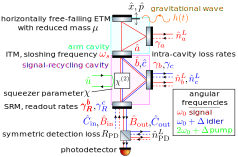
\includegraphics[width=\textwidth]{nIS_config.pdf}
	% squeezing ellipse and signal arrow plot
	\caption{\jam{(Draft figure, needs idler mode and labels)} Nondegenerate internal squeezing configuration, all modes are labelled. Showing the system's response using the signal arrow and noise ellipse representation from Fig.~\ref{}.}
	\label{fig:nIS_config}
\end{figure}

Nondegenerate internal squeezing consists of a nondegenerate squeezer placed inside the signal-recycling cavity of an interferometer, as shown in Fig.~\ref{fig:nIS_config} \jam{(have said this a few times already)}. In the single-mode approximation, I consider the signal and idler modes resonant in the signal-recycling cavity, where the signal mode of the squeezer is at the carrier frequency $\omega_0$ and is resonant in the arms, while the idler mode at $\omega_0+\Delta$ is assumed not resonant in the arms. 
I model this configuration using the Hamiltonian method demonstrated several times in this thesis, where this model combines the nondegenerate OPO model in Section~\ref{sec:nOPO} and the degenerate internal squeezing model in Section~\ref{sec:dIS_model}. There are no steps that have not already appeared in this thesis. This model is also based on and verified against Ref.~\cite{Li2020} in the lossless case. 
% \jam{(Probably need to talk about my methodology more -- state that this derivation presented is the last of a long line of increasing complexity (more losses, radiation pressure, pump phase, etc.) and that I have verified at each stage that the model recovers the previous model. This allowed me to also consider the impact of each subsequent addition in isolation. Moreover, I should re-emphasise that it reduces to the lossless case in Li and follows the same path as the verified models of dIS and the OPOs. The point is that this derivation is not controversial.)}
My methodology when constructing this model was to progressively add each complication to the lossless model in Ref.~\cite{Li2020}, such as optical loss in each mode, radiation pressure, and pump phase. At each stage, I verified that the model recovered the previous stage in the appropriate limits. This allowed me to study the effect of each complication one at a time, however, re-deriving the sensitivity each time was inefficient. I understand the sensitivity by looking at the signal and noise responses separately, and show all three whenever possible. \jam{(need to be more critical of the approach?)} I present the complete model here for brevity.

Let the modes be labelled as shown in Fig.~\ref{fig:nIS_config}, i.e.\ as in Section~\ref{sec:dIS_model} but with the addition of $\hat c$ for the idler mode as in Section~\ref{sec:nOPO}. The Hamiltonian of this system is $\hat H = \hat H_0 + \hat H_I + \hat H_\gamma + \hat H_\text{GW}$ where~\cite{} \jam{(fill in Langevin Hamiltonian)}
\begin{align}
\hat H_0 &= \hbar \omega_0 \hat a^\dag \hat a + \hbar \omega_0 \hat b^\dag \hat b+ \hbar (\omega_0+\Delta) \hat c^\dag \hat c + \hbar (2\omega_0+\Delta) \hat u^\dag \hat u\\
\hat H_I &= i\hbar\omega_s(\hat a\hat b^\dag-\hat a^\dag\hat b) + \hbar \frac{x}{2} (e^{i\phi} \hat u \hat b^\dag \hat c^\dag+e^{-i\phi} \hat u^\dag \hat b \hat c) \\
\hat H_\gamma &= \int \ldots \\
\hat H_\text{GW} &= -\alpha (\hat{x}-L_\mathrm{arm}h(t))(\frac{\hat{a}+\hat{a}^\dag}{\sqrt{2}})+\frac{1}{2\mu}\hat{p}^2.
\end{align}
As before, $\hat H_0$ describes the decoupled optical system, $\hat H_I$ describes the interaction between the three intra-cavity modes, $\hat H_\gamma$ describes the input/output coupling through the readout and loss ports listed below, and $\hat H_\text{GW}$ describes the coupling to the gravitational-wave signal and the evolution of the test mass mechanical mode.
There is vacuum entering the system intra-cavity to all three modes $\hat n^L_a, \hat n^L_b, \hat n^L_c$, at the readout port $\hat B_\text{in}, \hat C_\text{in}$, and in the detection chain $\hat n^L_\text{PD}$ which will be included later. Only the vacuum entering the readout port is present in the lossless model.
The Heisenberg-Langevin equations-of-motion for these operators can be found as before, using the bosonic and canonical commutation relations with all other commutators zero. I again (1) make the semi-classical and no-pump-depletion approximations to simplify the pump mode $\hat u\mapsto u=2\chi/x$, these approximations are valid below threshold, (2) enter the Interaction Picture to ignore $\hat H_0$, and (3) take fluctuating components of each operator but keep it implicit in the notation because it does not change the equations-of-motion \jam{(prove this?)}. I find the equations-of-motion to be
\begin{equation}
\begin{cases}
\dot{\hat{a}}=-\omega_s\hat{b} - \gamma_a \hat{a} + \sqrt{2\gamma_a}\hat{n}^L_a+\frac{i}{\hbar}\alpha(\hat{x}-L_\mathrm{arm}h)\frac{1}{\sqrt{2}}\\
\dot{\hat{b}}=\omega_s\hat{a} - i\chi e^{i\phi}\hat{c}^\dagger - \gamma^b_\mathrm{tot} \hat{b} + \sqrt{2\gamma^b_R}\hat{B}_\mathrm{in} + \sqrt{2\gamma_b}\hat{n}^L_b\\
\dot{\hat{c}}=-i\chi e^{i\phi}\hat{b}^\dagger - \gamma^c_\mathrm{tot} \hat{c} + \sqrt{2\gamma^c_R}\hat{C}_\mathrm{in} + \sqrt{2\gamma_c}\hat{n}^L_c\\
\dot{\hat{x}}=\frac{1}{\mu}\hat{p}\\
\dot{\hat{p}}=\alpha(\frac{\hat{a}+\hat{a}^\dag}{\sqrt{2}}).
\end{cases}
\end{equation}
I solve these equations in the Fourier domain with simplified notation $\tilde{\delta\hat{Q}}(\Omega)\mapsto\hat{Q}(\Omega)$. Let $\vec{\hat b}(\Omega)=[\hat b(\Omega), \hat b^\dag(-\Omega), \hat c(\Omega), \hat c^\dag(-\Omega)]^\text{T}$ with similar signal-idler vectorisation for each other mode as in Section~\ref{sec:nOPO} and $\vec{\hat a}(\Omega)=[\hat a(\Omega), \hat a^\dag(-\Omega),0,0]^\text{T},\quad \vec h(\Omega)=\tilde h(\Omega) [1,1,0,0]^\text{T}$ and similarly for $\vec{\hat n}^L_a(\Omega)$. Solving the resulting algebraic equations, I find that
\begin{align}
\mathrm{M}_b\vec{\hat{b}}(\Omega)&= \omega_s\begin{bsmallmatrix}
1 &  &  &  \\
 & 1 &  &  \\
 &  & 0 &  \\
 &  &  & 0
\end{bsmallmatrix}\mathrm{M}_a^{-1}\left(\sqrt{2\gamma_a}\begin{bsmallmatrix}
1 &  &  &  \\
 & 1 &  &  \\
 &  & 0 &  \\
 &  &  & 0
\end{bsmallmatrix}\vec{\hat{n}}^L_a(\Omega)-i\beta\begin{bsmallmatrix}
1 &  &  &  \\
 & -1 &  &  \\
 &  & 0 &  \\
 &  &  & 0
\end{bsmallmatrix}\vec{h}(\Omega)\right)\\&+ \sqrt{2}\begin{bsmallmatrix}
\sqrt{\gamma^b_R} &  &  &  \\
 & \sqrt{\gamma^b_R} &  &  \\
 &  & \sqrt{\gamma^c_R} &  \\
 &  &  & \sqrt{\gamma^c_R}
\end{bsmallmatrix}\vec{\hat B}_\mathrm{in}(\Omega) + \sqrt{2}\begin{bsmallmatrix}
\sqrt{\gamma_b} &  &  &  \\
 & \sqrt{\gamma_b} &  &  \\
 &  & \sqrt{\gamma_c} &  \\
 &  &  & \sqrt{\gamma_c}
\end{bsmallmatrix}\vec{\hat n}^L_b(\Omega)\\
\mathrm{M}_a &= (\gamma_a-i\Omega)\mathrm{I}+\frac{i\rho}{\Omega^2 \sqrt{2}}\begin{bsmallmatrix}
1 & 1 &  &  \\
-1 & -1 &  &  \\
 &  & 0 &  \\
 &  &  & 0
\end{bsmallmatrix}\\
\text{M}_b&=\begin{bsmallmatrix}
\gamma^b_\mathrm{tot} &  &  &  \\
 & \gamma^b_\mathrm{tot} &  &  \\
 &  & \gamma^c_\mathrm{tot} &  \\
 &  &  & \gamma^c_\mathrm{tot} 
\end{bsmallmatrix}-i\Omega \text{I}+\chi \begin{bsmallmatrix}
0 &  &  & i e^{i\phi} \\
 & 0 & -i e^{-i\phi} &  \\
 & i e^{i\phi} & 0 &  \\
-i e^{-i\phi} &  &  & 0
\end{bsmallmatrix}+\omega_s^2\begin{bsmallmatrix}
1 &  &  &  \\
 & 1 &  &  \\
 &  & 0 &  \\
 &  &  & 0
\end{bsmallmatrix}\text{M}_a^{-1}\begin{bsmallmatrix}
1 &  &  &  \\
 & 1 &  &  \\
 &  & 0 &  \\
 &  &  & 0
\end{bsmallmatrix}.
\end{align}
Where $\beta, \rho$ are from Eq.~\ref{eq:beta_and_rho}, $\text{I}$ is the 4 by 4 identity matrix, and all off-diagonal terms in each matrix are zero unless otherwise shown \jam{(is this clear or would it be better to include them explicitly?)}. Using $\Gamma= \frac{1}{\sqrt2}\begin{bsmallmatrix}
1 & 1 &  &  \\
-i & i &  &  \\
 &  & 1 & 1 \\
 &  & -i & i
\end{bsmallmatrix}$ and the input/output relations at the readout port and the detection loss port given by Eq.~\ref{eq:nOPO_IO_relations}, I find the signal and idler quadratures~\footnote{Where $\vec{\hat X}(\Omega)=[\hat X_{b,1}(\Omega),\hat X_{b,2}(\Omega),\hat X_{c,1}(\Omega),\hat X_{c,2}(\Omega)]^\text{T}$, as in Section~\ref{sec:nOPO}.} at the photodetector to be
\begingroup
\allowdisplaybreaks
\begin{align}
\vec{\hat X}_\mathrm{PD}(\Omega)&=\text{T}\vec h(\Omega)+\text{R}_\text{in}\vec{\hat X}_\mathrm{in}(\Omega)+\text{R}^L_a\vec{\hat X}^L_a(\Omega)+\text{R}^L_b\vec{\hat X}^L_b(\Omega)+\text{R}^L_\text{PD}\vec{\hat X}^L_\text{PD}(\Omega)\\
\text{T}&=-\sqrt{1-R_\text{PD}}\omega_s(-i\beta)\Gamma \sqrt{2}\begin{bsmallmatrix}
\sqrt{\gamma^b_R} &  &  &  \\
 & \sqrt{\gamma^b_R} &  &  \\
 &  & \sqrt{\gamma^c_R} &  \\
 &  &  & \sqrt{\gamma^c_R}
\end{bsmallmatrix}\text{M}_b^{-1}\begin{bsmallmatrix}
1 &  &  &  \\
 & 1 &  &  \\
 &  & 0 &  \\
 &  &  & 0
\end{bsmallmatrix}\text{M}_a^{-1}\begin{bsmallmatrix}
1 &  &  &  \\
 & -1 &  &  \\
 &  & 0 &  \\
 &  &  & 0
\end{bsmallmatrix}\\
\text{R}_\text{in}&=\sqrt{1-R_\text{PD}}\Gamma\left(\text{I}-2\begin{bsmallmatrix}
\sqrt{\gamma^b_R} &  &  &  \\
 & \sqrt{\gamma^b_R} &  &  \\
 &  & \sqrt{\gamma^c_R} &  \\
 &  &  & \sqrt{\gamma^c_R}
\end{bsmallmatrix}\text{M}_b^{-1}\begin{bsmallmatrix}
\sqrt{\gamma^b_R} &  &  &  \\
 & \sqrt{\gamma^b_R} &  &  \\
 &  & \sqrt{\gamma^c_R} &  \\
 &  &  & \sqrt{\gamma^c_R}
\end{bsmallmatrix}\right)\Gamma^{-1}\\
\text{R}^L_a&=-\sqrt{1-R_\text{PD}}\omega_s\Gamma 2\sqrt{\gamma_a}\begin{bsmallmatrix}
\sqrt{\gamma^b_R} &  &  &  \\
 & \sqrt{\gamma^b_R} &  &  \\
 &  & \sqrt{\gamma^c_R} &  \\
 &  &  & \sqrt{\gamma^c_R}
\end{bsmallmatrix}\text{M}_b^{-1}\begin{bsmallmatrix}
1 &  &  &  \\
 & 1 &  &  \\
 &  & 0 &  \\
 &  &  & 0
\end{bsmallmatrix}\text{M}_a^{-1}\begin{bsmallmatrix}
1 &  &  &  \\
 & 1 &  &  \\
 &  & 0 &  \\
 &  &  & 0
\end{bsmallmatrix}\Gamma^{-1}\\
\text{R}^L_b&=-\sqrt{1-R_\text{PD}}\Gamma 2\begin{bsmallmatrix}
\sqrt{\gamma^b_R} &  &  &  \\
 & \sqrt{\gamma^b_R} &  &  \\
 &  & \sqrt{\gamma^c_R} &  \\
 &  &  & \sqrt{\gamma^c_R}
\end{bsmallmatrix}\text{M}_b^{-1}\begin{bsmallmatrix}
\sqrt{\gamma^b_R} &  &  &  \\
 & \sqrt{\gamma^b_R} &  &  \\
 &  & \sqrt{\gamma^c_R} &  \\
 &  &  & \sqrt{\gamma^c_R}
\end{bsmallmatrix}\Gamma^{-1}\\
\text{R}^L_\text{PD}&=\sqrt{R_\text{PD}} \text{I}.
\end{align}
\endgroup
The total quantum noise is given by the spectral density matrix Eq.~\ref{eq:total_noise_matrix}, which simplifies, assuming uncorrelated vacuum at each loss port, to
\begin{equation}
\text{S}_X=\text{R}_\text{in}\text{R}_\text{in}^\dag+\text{R}^L_a{\text{R}^L_a}^\dag+\text{R}^L_b{\text{R}^L_b}^\dag+\text{R}^L_\text{PD}{\text{R}^L_\text{PD}}^\dag.
\end{equation} % same expression as dIS
Which is divided into 2 by 2 blocks of signal-signal, signal-idler, and idler-idler (co)variances as in Section~\ref{sec:nOPO}.
The vector of signal transfer functions, with respect to $\tilde h(\Omega)$, to each signal and idler quadrature at the photodetector is
\begin{equation}
\text{T}\begin{bsmallmatrix}1 \\1\\0\\0\end{bsmallmatrix} = \frac{2 \beta \sqrt{1-R_\text{PD}} \omega_s}{(\gamma_a-i \Omega ) \left(\chi ^2-(\gamma^b_\text{tot}-i\Omega) (\gamma^c_\text{tot}-i\Omega)\right)-\omega_s^2 (\gamma^c_\text{tot}-i \Omega )} \begin{bsmallmatrix}0 \\-\sqrt{\gamma^b_R}(\gamma^c_\text{tot}-i\Omega)\\\sqrt{\gamma^c_R}\chi\cos(\phi)\\\sqrt{\gamma^c_R}\chi\sin(\phi)\end{bsmallmatrix}.
\end{equation}
Therefore, there is gravitational-wave signal in the second signal quadrature and each idler quadrature. For simplicity and to compare to Ref.~\cite{Li2020}, here I will consider measuring the second signal quadrature which I will refer to as signal readout, henceforth. However, this is not necessarily the optimum readout of the signal quadratures since the noise might be sufficiently lower in the first quadrature to preference a combined measurement. I will consider this and other readout schemes, such as measurements of the idler quadratures and combinations of the signal and idler quadratures, like in Section~\ref{sec:nOPO_combined_readout}, in Chapter~\ref{chp:idler_readout}.
Therefore, the sensitivity of the signal readout scheme, where $\sqrt{S_h}$ is the noise-to-signal ratio, is
\begin{equation}
S_h = \frac{(\text{S}_X)_{2,2}}{\abs{\left(\text{T}\begin{bsmallmatrix}1 \\1\\0\\0\end{bsmallmatrix}\right)_2}^2}.
\end{equation}
% verified these results by repeating the model with 2x2 matrices and 4x4 matrices, important to mention this because it is part of the methodology
I have verified this result by repeating the derivation, instead using 2 by 2 matrices~\footnote{This is not a physically meaningful difference, but it separates the signal and idler such that the derivations are not identical.}, and will also compare it to known limits below. %in Section~\ref{sec:nOPO_reduction}.


\section{Results}

\subsection{General performance}

\jam{(continue from here)}

% explain the effect of each parameter (except leave tolerance to losses to science case chapter)

% should this be down in results section? --> this is a results chapter, maybe include a short section discussing the general performance (separate from the science case analysis in chapter 5?)
% analyse typical nIS plot features before getting into different tests
% plot: classic N, S, NSR; also noise budget plot
% need to show some example plots here to set up those in the next section?
\begin{figure}
	\centering
	\includegraphics[width=\textwidth]{nIS_N_S_NSR.pdf}
	\caption{Nondegenerate internal squeezing quantum noise and signal responses, and sensitivity.}
	\label{fig:}
\end{figure}

\begin{figure}
	\centering
	\includegraphics[width=\textwidth]{nIS_sigRO_noise_budget.pdf}
	\caption{Nondegenerate internal squeezing breakdown of quantum noise sources, plotting separate noise transfer functions for each loss port (this is akin to a typical ``noise budget''~\cite{} but not quite the same).}
	\label{fig:}
\end{figure}


\subsection{Reduction to known systems}
\label{sec:nOPO_reduction}

% show that this follows from the EoM but can be verified by looking at the plots

\subsubsection{Lossless, PT-symmetric limit}

\begin{figure}
	\centering
	% \includegraphics[width=\textwidth]{}
	\caption{Nondegenerate internal squeezing sensitivity showing the lossless limit. \jam{(Could be already covered in nISNSNSR.pdf use code from Li et al 2020, Fig 5 to make comparison really convincing)}}
	\label{fig:}
\end{figure}

\jam{(factor of 2 disagreement with Li in result?)}
% symmetry broken by losses and RP, repair by BAE but too complicated for here

\subsubsection{Nondegenerate OPO limit}
\begin{figure}
	\centering
	\includegraphics[width=\textwidth]{nIS_nOPO_limit.pdf}
	\caption{Nondegenerate internal squeezing shot noise response (i.e. quantum noise with radiation pressure turned off) showing the large arm loss limit.}
	\label{fig:}
\end{figure}

% give best explanation of ITM T=0, but can admit that while the maths is clear the physics is not obvious -- potentially requires more thought

% therefore mystery of the idler loss carries over: idler loss cannot be zero

% full 4x4 matrix agrees, not just variance 1,1

\subsection{Stability}

% will need to review stability

% plot: imaginary part of poles
\begin{figure}
	\centering
	\includegraphics[width=\textwidth]{nIS_stability.pdf}
	\caption{Stability of nondegenerate internal squeezing, showing the imaginary part of the poles of the transfer functions, when the imaginary part becomes positive the system becomes unstable~\cite{}.}
	\label{fig:}
\end{figure}

% effect of RP, pump phase

\section{Singularity threshold}
\label{sec:singularity_threshold}

\jam{(Emphasise that this is original work and that it is a clever approach.)}

% motivate this by the previous section's looking at poles, now looking at real poles that could be encountered, to avoid confusion with the complex poles that are always present I will call these real poles ``singularities''

% $\Omega^2$ factor in RP denominator is the resonance, but is unrelated to the squeezer



I have devised a definition of threshold: ``threshold is the (real) value of the squeezing parameter such that the anti-squeezed quadrature of the quantum noise has a singularity at some (real) frequency; if multiple singularities exist then the threshold is the smallest squeezer value''. Here, I am only looking for singularities that diverge to infinity (along all angles of approach). In order to reduce confusion, I do not call these ``poles'' since the quantum noise is not defined on $\mathbb{C}$. \jam{(Check this: looking at the imaginary part of the poles for stability and looking for real poles (i.e. poles on the real axis) for threshold are the same solutions, surely?)}
% NB: I am calling the points "singularities" for now to avoid confusion, but they are just the poles of the transfer functions (against complex \[CapitalOmega]) at real \[Chi] such that they are on the real axis (and therefore real \[CapitalOmega]).

For this unified, anti-squeezed singularity definition of threshold, I find the real singularities of each system to be at:
\begin{align}
\label{eq:unified-threshold}
\mathrm{dOPO}&: \Omega=0, \chi=\gamma^b_\mathrm{tot}\\
\mathrm{nOPO}&: \Omega=0, \chi=\sqrt{\gamma^b_\mathrm{tot}\gamma_c}\\
\mathrm{dIS}&:\begin{cases}
\Omega=0, \chi=\gamma^b_\mathrm{tot}+\frac{\omega_s^2}{\gamma_a};&\gamma_a\neq0\\
\Omega=\sqrt{\omega_s^2-\gamma_a^2}, \chi=\gamma^b_\mathrm{tot}+\gamma_a;&\omega_s\geq\gamma_a\geq0
\end{cases}\\
\mathrm{nIS}&:\begin{cases}
\Omega=0, \chi=\sqrt{\gamma_c(\gamma^b_\mathrm{tot}+\frac{\omega_s^2}{\gamma_a})};&\gamma_c\neq0,\gamma_a\neq0\\
\Omega=\sqrt{\frac{\gamma_c\omega_s^2+\gamma_a(-\omega_s^2-\gamma_a(\gamma^b_\mathrm{tot}+\gamma_c))}{\gamma^b_\mathrm{tot}+\gamma_c}}, \chi=\sqrt{(\gamma_a+\gamma^b_\mathrm{tot})(\gamma_a+\gamma_c+\frac{\omega_s^2}{\gamma^b_\mathrm{tot}+\gamma_c})};&\gamma_c\neq0,(*)
\end{cases}\\
(*)&:\gamma_c\omega_s^2\geq\gamma_a\omega_s^2+\gamma_a^2(\gamma^b_\mathrm{tot}+\gamma_c)
\end{align}

For dIS, by Eq.~\ref{eq:unified-threshold}, the definition reduces to dOPO threshold $(\Omega,\chi)\xrightarrow[\gamma_a\rightarrow\infty]{}(0,\gamma^b_\mathrm{tot})$ and to the lossless threshold $(\Omega,\chi)\xrightarrow[\gamma_a\rightarrow0]{}(\omega_s,\gamma^b_\mathrm{tot})$.
For nIS, this definition reduces to nOPO threshold $(\Omega,\chi)\xrightarrow[\gamma_a\rightarrow\infty]{}(0,\sqrt{\gamma^b_\mathrm{tot}\gamma_c})$ and to the lossless threshold in the formal limit $(\Omega,\chi)\xrightarrow[\gamma_a=0,\gamma_c\rightarrow0]{}(0,\omega_s)$. This last limit makes sense from the stability \jam{(make sure stability already studied)} analysis, since the lossless system is marginally stable at threshold and this anti-squeezed singularity definition looks for when the poles are on the real axis.

Radiation pressure and back-action evasion do not change threshold because the quantum noise transfer function denominator has the same positive zeros as the shot noise transfer function without radiation pressure (and BAE).
% pump phase does not change threshold either

% this resolves the mystery of idler loss --> means that lossless nIS is necessarily above threshold and therefore not allowed in this model except in formal limits, pump depletion would need to be added in to properly compare to sWLC



\begin{figure}
	\centering
	% \includegraphics[width=\textwidth]{}
	\caption{Sensitivity of configurations on threshold. \jam{(Is this necessary, instead just reference plots in other chapters?)}}
	\label{fig:}
\end{figure}

\begin{figure}
	\centering
	\includegraphics[width=\textwidth]{nIS_threshold.pdf}
    \includegraphics[width=\textwidth]{dIS_threshold.pdf}
	\caption{Trajectory of singularities in (real) $(\Omega, \chi)$ space as losses are changed for nondegenerate internal squeezing (left) and, for reference, for degenerate internal squeezing (right). Degenerate and nondegenerate OPO behaviour is not interesting as thresholds remain at DC ($\Omega=0$) and are relatively simple: $\sqrt \gamma^b_\text{tot}$ and $\sqrt \gamma^b_\text{tot} \gamma^c_\text{tot}$, respectively.}
	\label{fig:}
\end{figure}

% plot: OPO and lossless dIS, nIS on threshold
% plot: trajectory of poles for lossy dIS and nIS -- maybe cut dIS because nIS should be the focus? 


\subsection{Problems with definition}

% make clear that knowing threshold just gives the physical bounds of the parameter space, it doesn't correspond to the optimal squeezing (see results section) for sensitivity improvement -- just as minimising N does not necessarily maximise SNR if signal is not considered. 

\subsubsection{Disagreement between squeezed and anti-squeezed quadratures}
% Degenerate internal squeezing - different notions of threshold
%shouldn't this be in the dIS sub-chapter? no.

% plot: both quadratures comparison (black-green plot)

\begin{figure}
	\centering
	\includegraphics[width=\textwidth]{dIS_threshold_quadratures.pdf}
	\caption{Degenerate internal squeeing difference between singularity threshold (that maximises anti-squeezing peak) and squeezing parameter that minimises peak squeezing.}
	\label{fig:}
\end{figure}

\jam{(One explanation for the difference between position of the singularity of the anti-squeezed quadrature and the minimum of the squeezed quadrature is that the expression for the sloshing frequency in Korobko et al, 2019 is not valid at large arm losses. If this is so, then what does this fixed--sloshing frequency Hamiltonian correspond to? And for that system, why does the supposedly Gaussian squeezing not maximise antisqz at the frequency that it minimises squeezing? --> Look at pump phase and/or covariance matrix)}



% \subsection{PT-symmetry}
% % mention removing back-action evasion

\subsection{Physical meaning of singularity threshold}
% Preliminary work? should be subsubsection?

% will this all evaporate when pump depletion is added? yes, its likely

% \section{Tolerance to optical losses}
% this is repeated in the next chapter? but I need this to explain the behaviour with different readout?



%%%%%%%%%%%%%%%%%%%%%%%%%%%%%%%%%%%%%%%%%%
\section{Chapter summary}


\jam{(Have I been critical of my approach?)}



%%%%%%%%%%%%%%%%%%%%%%%%%%%%%%%%%%%%%%%%%%
\chapter{Gravitational-wave detection science case for nondegenerate internal squeezing}
\label{chp:science_case}
% comparison to existing proposals

% be clear about the scope of this project, I am not wanting to recommend the design of the next detector to be built, this is exploratory work into a configuration that has never been modelled this thoroughly before -- more would need to be done (e.g. add in external squeezing and thermal noise etc.) to make a proper judgement which is not my aim.

\section{Experimental constraints} %on parameter space

% will need to decide on a parameter set to make the rest of the plots: use LIGO Voyager at different readout rates? use the Li data set which is this already?

% IFO parameter space -- Pcirc is fixed

% what are realistic losses, what are ideal losses?

% table: parameter sets to compare
\begin{table}
	\caption{Table of interferometer parameter sets, showing configuration and derived parameters. The parameter set from Ref.~\cite{} is based on LIGO~Voyager but directly sets the readout rate $\gamma_R$ and sloshing frequency $\omega_s$ and back-forms the corresponding physical lengths and reflectivities. \jam{(Freedoms in this process)}}
	\label{tab:}
\end{table}

\section{Results}


\subsection{Tolerance to optical loss}
% plot: tolerance to each of the four sources, matrix plot each against readout rate
% some way to mega matrix all of these, or just show sensitivity and not N and S separetely?
\begin{figure}
	\centering
	\includegraphics[width=\textwidth]{nIS_sigRO_tolerance_Rpd.pdf}
	\caption{Nondegenerate internal squeezing tolerance to loss (1/4): detection loss.}
	\label{fig:}
\end{figure}
\begin{figure}
	\centering
	\includegraphics[width=\textwidth]{nIS_sigRO_tolerance_Tlb.pdf}
	\caption{Nondegenerate internal squeezing tolerance to loss (2/4): signal mode, intra-cavity signal-recycling cavity loss.}
	\label{fig:}
\end{figure}
\begin{figure}
	\centering
	\includegraphics[width=\textwidth]{nIS_signalRO_tolerance_Tlc.pdf}
	\caption{Nondegenerate internal squeezing tolerance to loss (3/4): idler mode, intra-cavity signal-recycling cavity loss.}
	\label{fig:}
\end{figure}
\begin{figure}
	\centering
	\includegraphics[width=\textwidth]{nIS_sigRO_tolerance_Tla.pdf}
	\caption{Nondegenerate internal squeezing tolerance to loss (4/4): intra-cavity arm cavity loss.}
	\label{fig:}
\end{figure}

% resistant to detection losses, which is a big deal, although Caves's amplifier could alleviate this more generally
% resistant to signal loss, sensitive to arm loss, very sensitive to idler loss (SRM must be closed to idler through e.g. dichroic)




\subsection{Optimal squeezing}

\begin{figure}
	\centering
	\includegraphics[width=\textwidth]{nIS_optimum_squeezing.pdf}
	\caption{Nondegenerate internal squeezing optimal squeezing curve for sensitivity at probe frequency, i.e.\ plotting sensitivity and noise measured at a particular ``probe'' frequency for varying squeezing parameters and different detection losses.}
	\label{fig:}
\end{figure}

% plot optimal squeezing curve (blue-green swoosh)
% mention that this can be done for probe frequency, peak frequency, integral etc.

% emphasise that threshold is not optimal squeezing for sensitivity

\section{Feasibility for gravitational-wave detection}

% stress that the goal of this thesis is not to provide a recommendation to the designers of future gravitational wave detectors of what parameters to use, that task is much harder and would require the modelling of many other effects. This section (and thesis) is only exploratory in nature, and my conclusion is that nIS warrants more study because it appears to be able to get close enough to the targets (without increasing power) and is comparable to optomechanical alternative, and more resistant to detection losses than degenerate internal squeezing (operated in the squeezing not anti-squeezing pump phase).

% miao et al, 2018 astro target and mutrics

% directly address the vagueness with ``is this configuration useful to GW detection'', talking about a particular parameter set or the best param set possible?

% motivation was kilohertz detection but works better as broadband detector?
% cover two detector designs

    % Sensitivity target of 5e-25 from 1--4 kHz.
    % 	With high squeezer ratio, i.e. 95\%, and ideal losses, then target can be hit for less than 1kHz of the band. With even higher squeezer ratio, i.e 99\%, and increased omegaS to move the peak into kHz (and corresponding increased gammaR), then the target can be hit for 1--3kHz.
    % 		Bottom line: nIS can achieve the sensitivity target partially across the band, with more and more ideal conditions/optimisation of omegaS and gammaR necessary to widen the range that it achieves it at.
    % 		Recommending a detector design isn't the goal of my project, but I do want to say something re: the sensitivity target. Right now, it sounds like nIS can achieve it at some peak frequency (under ideal conditions) but not from 1--4kHz for a Voyager-like detector.


\subsection{Application to kilohertz detection}

\begin{figure}
	\centering
	% \includegraphics[width=\textwidth]{nIS_ideal_losses.pdf}
	\caption{\jam{(Add in curve with more realistic losses)} Nondegenerate internal squeezing sensitivity under ideal conditions, and under more realistic conditions. The sensitivity target (shown in red) can perhaps be achieved at a peak frequency but not realistically across the 1--4~kHz band. These conditions are for fixed circulating power in the arm cavity and no external squeezing.}
	\label{fig:}
\end{figure}

% plot: curve optimised for kilohertz

% need to show curve

% achieving target across the band looks very unlikely, but target might be achievable at a particular kilohertz frequency
% note the limitations with the target (conditions on a particular EoS of the neutron star etc.)

% mention mutricK's for optimisation? don't need to put everything in the thesis
% plot: curve optimised for mutricK?

% this is without external squeezing


\subsection{Application to broadband detection}
% optimisation?

\begin{figure}
	\centering
	% \includegraphics[width=\textwidth]{}
	\caption{Nondegenerate internal squeezing sensitivity optimised for broadband detection (i.e.\ with integrated sensitivity from 0 to $\infty$ optimised).}
	\label{fig:}
\end{figure}
% plot: curve optimised for broadband 

% kilohertz detection was the aim of the thesis but it looks like nIS might be more useful for a different purpose, set up idler readout chapter

% \section{Sensitivity optimisation}

% % chosen metrics (mutrics), optimisation to hit astrophysical target
% % Realistic experimental constraints



\section{Comparison to existing proposals}

\subsection{All-optical versus optomechanical configuration}

\begin{figure}
	\centering
	\includegraphics[width=\textwidth]{nIS_compared_to_singleCav.pdf}
	\caption{\jam{(Add in curves from Li et al, 2020 Fig. 5 notebook)} Nondegenerate internal squeezing compared to stable optomechanical filtering. Errant \jam{(word choice)} factors of two in the sensitivity (perhaps from the scalar versus vector convention of the signal transfer function) and in the test mass mass (perhaps from different conventions of the reduced mass) are required. Uses data from Ref.~\cite{} with direct permission from the authors.}
	\label{fig:}
\end{figure}

% don't overlay Fig. 5 from Li et al, 2020
% plot: with data from Fig. 5 in Li --> extract the plot and don't mess with the .nb further!
    % The key result is that I've found losses for nIS that replicate the results for sWLC: arm loss 75 ppm, idler loss 100 ppm. For these ideal losses, the peak sensitivity and bandwidth are better than sWLC.
	   %  Are these loss values more realistic than the thermal and mechanical constraints of sWLC? I think so, but I need back-up on this.
% all-optical approach is at least comparable to optomechanical approach

% \subsubsection{}
% The problem with making a judgement
% emphasise that this result is not a clean decision, the best I can say is that they are comparable
% forcasting future technological progress is hard to do rigourously or scientifically

% ultimately: is the all-optical approach viable? yes!

% do I need to include this? it would be nice --> above comparison is the focus though
\subsection{Degenerate versus nondegenerate internal squeezing}
% degenerate internal squeezing can be run in amplification regime if losses are high
% nondegenerate is less sensitive to losses and could potentially use idler/combined readout to get ahead --> next chapter


%%%%%%%%%%%%%%%%%%%%%%%%%%%%%%%%%%%%%%%%%%
\section{Chapter summary}





%%%%%%%%%%%%%%%%%%%%%%%%%%%%%%%%%%%%%%%%%%
\chapter{Idler and combined readout schemes for nondegenerate internal squeezing}
\label{chp:idler_readout}
% only a short chapter!

% justify why this is a separate chapter

% section 3-B in Li 2021 has noticed this already! --> but their idler has to read out the mechanical mode!

% chronological does not matter, make this flow from the previous chapter --> emergence of a new possibility separate from initial interest in kilohertz sensitivity

\jam{(how preliminary is this work? I understand idler readout's threshold, stability, limits, tolerance to losses, and performance against readout rates. no, I don't physically understand the profile, but I have a lot of characterisation)}

\section{Analytic model}
% short section
% review idler and combined signal-idler readout from nOPO chapter


\section{Results}
% mirror chapters 4,5

\subsection{Stability and threshold}

% stability and singularity threshold maintained (same denominator)


\subsection{Reduction to OPOs}

% reduction to nOPO and dOPO (recovers squeezing)

\begin{figure}
	\centering
	% \includegraphics[width=\textwidth]{}
	\caption{Nondegenerate internal squeezing, idler readout recovers nondegenerate OPO (also shows tolerance to arm cavity intra-cavity loss).}
	\label{fig:}
\end{figure}

\begin{figure}
	\centering
	\includegraphics[width=\textwidth]{nIS_combinedRO_dOPO_limit.pdf}
	\caption{Preliminary work: combined signal-idler readout, showing the limit of large arm loss that recovers a degenerate OPO (in the same manner that the nondegenerate OPO Weiner filter recovers a degenerate OPO, shown in Section~\ref{}). \jam{(Just show noise response?)}}
	\label{fig:}
\end{figure}

% interesting that combined nIS does not reduce to dIS, perhaps this is because the idler is not resonant in the arms

% split into own section?
\subsection{Idler readout tolerance to losses}

% why focus on idler readout, combined readout is largely left to future work

% idler readout tolerance to losses (showcase preliminary results)
% decrease in peak sensitivity, large increase in bandwidth
\begin{figure}
	\centering
	\includegraphics[width=\textwidth]{nIS_idlerRO_tolerance_Tlb.pdf}
	\caption{Nondegenerate internal squeezing, idler readout tolerance to signal mode intra-cavity loss.}
	\label{fig:}
\end{figure}

\begin{figure}
	\centering
	\includegraphics[width=\textwidth]{nIS_idlerRO_tolerance_Tlc.pdf}
    \includegraphics[width=\textwidth]{nIS_idlerRO_tolerance_Rpd.pdf} 
	\caption{Nondegenerate internal squeezing, idler readout tolerance to idler and detection losses. \jam{(Separate figures)}}
	\label{fig:}
\end{figure}

% tolerance to losses? see problem with position of signal readout tolerance above

\subsection{Idler readout tolerance to pump power and phase}
% stability of idler readout against pump power and phase: how sensitive is the scheme to ratio of threshold and $\phi$ (when $\psi$ combination angles fixed), give value in $\%$ and radians.


\begin{figure}
	\centering
	\includegraphics[width=\textwidth]{nIS_ROs_tolerance_chi.pdf} % mention what happens when idler readout rate is kept high and signal rate is varied, see nIS_ROs_tolerance_chi_large_idler_ROrate.pdf
	\caption{Nondegenerate internal squeezing, idler readout tolerance to pump power (squeezer parameter $\chi$).}
	\label{fig:}
\end{figure}

% idler readout transfer functions: noise indep of pump phase but noise dep on relative phase of pump to linear combination of idler quadratures

\begin{figure}
	\centering
	\includegraphics[width=\textwidth]{nIS_ROs_tolerance_phi.pdf}
	\caption{Nondegenerate internal squeezing, idler readout tolerance to pump phase $\phi$ with combination angle $\psi_1$ fixed, compared to signal readout's tolerance. \jam{(sequencing of plots?)}}
	\label{fig:}
\end{figure}

% check squeezing?


\section{Idler readout comparison to signal readout}

% section 3-B in Li 2021 has noticed this already! ``In the course of this work, I became aware of a related result in Ref.~\cite{Li2021} for the optomechanical analogue of this configuration.''


% plot: separate idler and signal readout, reduction to OPOs, combined reduction to dOPO
% tradeoff of bandwidth and DC peak sensitivity + interaction with RP
\begin{figure}
	\centering
	\includegraphics[width=\textwidth]{nIS_signal_vs_idler_ROs.pdf}
	% why is the peak moving? threshold should not be a factor since ratio fixed?
	% showcase same lines without RP?
	\caption{Idler readout compared to signal readout. Idler readout appears promising at lower-than-kilohertz frequencies around $100$~Hz, especially when the readout rates are comparable. \jam{(check whether incoherent readout is possible when the modes are correlated, does measurement collapse the entanglement?)}}
	\label{fig:}
\end{figure}

% is this true: These readout schemes can not be run simultaneously due to measurement collapsing the entangled state of the signal and idler -- ``independent'' readouts here refers to if each was run separately?

% The latest idler readout plots:
% (Plot 1) Dashed lines are without radiation pressure. The result is that the signal transfer function improvement with idler readout persists at low frequencies but radiation pressures means that there's no sensitivity improvement. 
% (Plots 2-3) Zoom-in on peak frequency, which changes with the readout rate. This is because the singularity threshold frequency depends on the losses, although I normalise the squeezer parameter to the singularity threshold value I don't normalise the frequency axis. The singularity frequencies here are: {853, 1624, 3534, 4763} Hz (truncated at the decimal point). Plot 2 is for 95% of the squeezer parameter threshold; Plot 3 is on squeezer parameter threshold (where limited resolution means that the peak is finite). When the signal readout is turned off, the effect is smaller but non-zero.
% (Plots 4-5) Tolerance to pump power. Showing the effect of changing the ratio to threshold by plus/minus 4%. The effect appears larger at smaller idler readout rates with fixed signal readout rate (Plot 4) and negligible when idler readout is large and signal readout is varied (Plot 5). I suspect that this is due to the likeness to the lossless case with no idler readout (Li et al, 2020) where 100% threshold is dramatic compared to 90% threshold -- compared to at large readout rates where 90 and 100% threshold are largely the same. Why low signal readout does not produce the same effect is because it is further from that lossless configuration, but I am less confident about this.
% The regime that is most promising is for readout rates roughly equal, so this effect for low idler readout's is less of an issue, and it appears similar to the signal readout anyway. 
% (Plot 6) Tolerance to pump phase. Fixing the combination angle psi1=pi/2 and changing the pump phase phi from pi/2 by plus/minus pi/4. Plot 6 is labelled as "combined" but the angles are selecting idler readout only. The effect is that the sensitivity seems tolerant to pump phase, independently of the readout rates (which surprised me, recall that psi1=phi is optimal for signal but the change is small). 

\section{Gravitational-wave sub-kilohertz detection science case for idler readout}

% idler readout also looks quite promising but demands a lot more investigation before drawing strong conclusions, need to be critical of my methodology and approach
% nondegenerate is less sensitive to losses and could potentially use idler/combined readout to get ahead

\begin{figure}
	\centering
	% \includegraphics[width=\textwidth]{}
	\caption{Nondegenerate internal squeezing, idler readout for LIGO~Voyager parameter set for losses with different levels of realism and different readout rates, compared against sensitivity target.}
	\label{fig:}
\end{figure}

% showcase the reasons for further interest in this configuration
% Since $\Delta$ does not affect the sensitivity as long as $\Delta \ll \omega_0$, the idler frequency can be chosen to best suit the current photodetector technology, e.g.\ photodiodes at $2 \mu\text{m}$ suffer from low quantum efficiency~\cite{} so although the signal mode might be at $2 \mu\text{m}$ for separate reasons~\cite{}, the idler wavelength can be chosen to optimise the readout.
% David Ottaway: the frequencies where the idler is improving low freq sensitivity might fit into the band of InGaaAs photodetectors where the sensitivity at 2 um can be improved (currently this is a problem i.e low Quantum efficiency of photodetectors at 2um) - Vaishali

\begin{figure}
	\centering
	% \includegraphics[width=\textwidth]{}
	\caption{Preliminary work: nondegenerate internal squeezing, combined readout for LIGO~Voyager parameter set for losses with different levels of realism and different readout rates, compared against sensitivity target.}
	\label{fig:}
\end{figure}

% combined (coherent) readout is even more interesting than swapping between signal and idler readout because the correlations can be used to potentially achieve even greater sensitivity
% give a sense that this exploration is not yet finished but is quite promising




%%%%%%%%%%%%%%%%%%%%%%%%%%%%%%%%%%%%%%%%%%
\section{Chapter summary}




